\graphicspath{{chapters/images/0202/}}

\chapter{Statistical decision theory}
  
  \section{Definition of statistical decision theory}
    The \textbf{statistical decision theory} is a set of quantitative methods for reaching optimal decisions for well posed problems. Statistical decision theory applies to supervised learning, while it does not apply to unsupervised learning. For most of the course we will focus on supervised learning (\href{https://www.britannica.com/science/decision-theory-statistics}{decision theory statistics from Britannica}). 

  \section{Supervised learning}
    \textbf{Supervised learning} is a set of methods whose objective is, given the observations $(\vec{x}_i, y_i)$ with $i = 1, \dots, n$, to \textbf{find a rule $\hat{f}$ that allows us to predict $Y$ from $\vec{X}$}, meaning that $\hat{Y} = \hat{f}(\vec{X})$. $\hat{f}(\vec{X})$ is thus an approximation of the true rule $f(\vec{X})$. Finding $\hat{f}$ corresponds to training (or fitting) a model using labelled data pairs (both predictors and response values are known).

    Broadly, there are two main types of methods of supervised learning: 
    \begin{itemize}
      \item \textbf{Regression methods}, in which the response $Y$ is quantitative (numerical). In this case $\hat{f}$ is called \textbf{regression function}.
      \item \textbf{Classification methods}, in which the response $Y$ is qualitative (categorical). In this case $\hat{f}$ is called \textbf{classifier}.
    \end{itemize}
    
    The predictors ($\vec{X}$) can take any form, numerical or categorical. In general there are no assumptions on the form of the predictors (but not always).
    
    To evaluate a model you use \textbf{loss functions}, which are functions used to penalize the differences between $Y$ and $f(\vec{X})$. Many loss functions can be used; the choice of a specific loss function determines which function is considered to be the true rule $f(\vec{X})$.

  \section{Regression setting}
    In a regression setting, the loss function which is generally used is the \textbf{squared error loss function} (also referred as the risk of estimating $ Y $ using $ f(\vec{X}) $), which is defined as
    $$L(Y,f(\vec{X})) = (Y-f(\vec{X}))^2$$
    When using this loss function, the criterion for choosing the model becomes finding $f$ such that it minimizes the \textbf{expected prediction error} (EPE), which is the expected value of the squared error loss function:
    \begin{align*}
      \text{EPE}(f) & = E_{Y,\vec{X}}[(Y-f(\vec{X}))^2] \\
                    & = \iint (y - f(\vec{x}))^2 g_{Y,\vec{X}}(y, \vec{x})\,dy\,d\vec{x} & \text{if } Y \text{ is continuous}
    \end{align*}
    This error is an expectation since you usually do not know the distribution of $Y$ and $\vec{X}$.
    If Y is continuous you can rewrite this expectation as the double integral times the joint density function $g$.\\
    
    \begin{theorem}[Minimum of the expected prediction error]
      $\text{EPE}(f) = E_{Y,\vec{X}}[(Y-f(\vec{X}))^2]$ has a \textbf{minimum} when 
      $f(\vec{x}) = E[Y|\vec{X} = \vec{x}]$.
      $f(\vec{x})$ is called regression function.
    \end{theorem}
    % TODO Maybe it is needed to add pedices to the expectations

    \begin{proof}
      (Sketch)
      By definition we know that
      $$\text{EPE}(f) = E_{Y,\vec{X}}[(Y-f(\vec{X}))^2]$$

      Then, since the law of \textit{iterated expectations} states that the expected value of a random variable is equal to the sum of the expected values of that random variable conditioned on a second random variable, so $E[X] = E[E[X|Y]]$, we get 

      $$E_{Y,\vec{X}}[(Y-f(\vec{X}))^2] = E_{\vec{X}}[E_{Y|\vec{X}}[(Y-f(\vec{X}))^2| \vec{X}]$$
      
      If we then consider a specific value of $\vec{X}$, meaning $\vec{X} = \vec{x}$, the inner expectation becomes 
      
      $$E[(Y-f(\vec{x}))^2 | \vec{X} = \vec{x}\,] $$
      
      But since $\vec{x}$ is fixed, $f(\vec{x})$ is a constant, hence this expectation can be written as a function in some parameter $a$

      $$g(a) = E_{Y}[(Y-a)^2]$$

      Then we want to find the (constant) value of $a$ that minimizes $g(a)$
      \begin{align*}
        g(a) & = E_{Y}[(Y-a)^2]               & \\
             & = E[Y^2 - 2aY + a^2]           & \text{compute the square} \\
             & = E[Y^2] -2aE[Y] + E[a^2]      & \text{separate expectations} \\
             & = E[Y^2] -2aE[Y] + a^2         & \text{pull out } a^2 \text{ since constant} \\
      \end{align*}

      Then, setting the derivative to zero we get 

      $$\frac{dg}{da} = -2E[Y] + 2a \mbeq 0 \implies \hat{a} = E[Y]$$

      Notice that if you plug $\hat{a}$ into $g(a) = E_{Y}[(Y-a)^2]$ you get

      $$g(\hat{a}) = E_{Y}[(Y-E[Y])^2] = Var(Y)$$
      
      Since $a = E[Y]$, the function that minimizes the $ g(a) $ function and consequently the EPE is 

      $$f(\vec{x}) = E[Y|\vec{X} = \vec{x}]$$
    \end{proof}
    % TODO Some steps could be clearer

    In a regression setting you could use other loss functions, such as the \textit{absolute error loss} function
    $$L(Y|f(\vec{X})) = |Y - f(\vec{X})|$$
    which is used in \textbf{least absolute deviation} (LAD) regression. In this case $f(\vec{x})$ is the median of $Y$ given $\vec{x}$, therefore you have a model which is more robust to outliers.

    We will choose the squared error loss and this motivates how the methods are developed.
    For example:
    \begin{itemize}
      \item \textbf{Linear regression} (parametric regression) can be expressed as 
            $$Y|\vec{X} = \vec{x} \sim N(\vec{x}^t\vec{\beta}, \sigma^2)$$ 
            or focussing more on the conditional mean
            $$E[Y|\vec{X} = \vec{x}] = \beta_0 + \beta_1x_1 + \dots + \beta_px_p$$
      \item \textbf{K-nearest neighbours regression}: one of the most used non-parametric regression
    \end{itemize}

    \subsection{K-nearest neighbours regression (KNN)}
    
      In the scope of regression, K-nearest neighbours method is defined as
      $$\hat{f}(\vec{x}) = \text{ Average } (y_i | \vec{x}_i \in N_K(\vec{x})) = \frac{1}{K} \sum_{x_i \in N_\vec{x}} {y_i} $$ %TODO modify the position of y_i
      Where:
      \begin{itemize}
        \item Average is the sample mean
        \item $N_K(\vec{x})$ is the neighbourhood of $K$ points closest to $\vec{x}$
      \end{itemize}

\begin{figure}[h]
\caption{The training data are shown in blue dots, test data and test data's predictions are star-shaped. The predicted value on test data is given making the average of the neighbours' values}
\centering
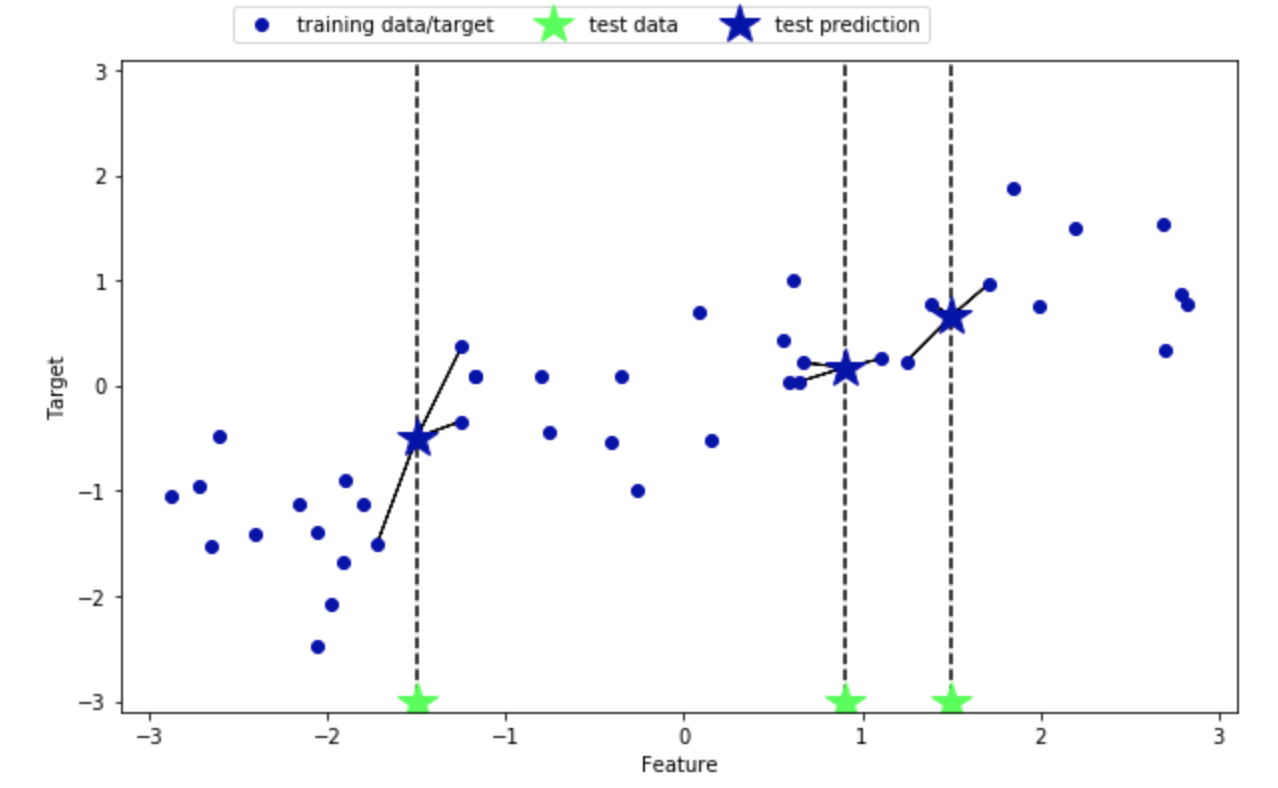
\includegraphics[width=0.6\textwidth]{KNNregression}
\end{figure}


      This method makes two approximations:
      \begin{itemize}
        \item It uses sample mean to approximate population mean
        \item It uses a neighbourhood of $\vec{x}$ rather than only $\vec{x}$
      \end{itemize}
      
      This method works well if you have a high amount of data and the number of parameters ($p$) is small.
      This simple method is rarely used, but it has inspired the development of more sophisticated kernel methods.

  \section{Classification setting}
    In a classification setting the response $Y$ is categorical, with $K$ categories. 
    A \textbf{classifier} is deciding which class to assign to a new observation $\vec{x}$.
    In this case $\hat{Y}$ is the predicted class.
    
    An example of loss function that can be used in classificiation setting is the \textbf{0-1 loss function} which penalizes classifying a datapoint in the wrong class. Assume for instance the binary case, meaning $K = 2$ (but you could generalize for any number of classes); in that case the 0-1 loss function can be represented as:
    
\begin{table}
\centering
\begin{tabular}{|l||c|c|}
	\hline
	\textbf{True,
	Predictions} & \textbf{0} & \textbf{1} \\
	\hline
	\hline
	\textbf{0} &  $0$ & $1$ \\
	\hline
	\textbf{\textbf{1}} & $1$ & $0$\\
	\hline
\end{tabular}
\caption{This is the table representing the possible values of $ L(Y, \hat{Y}(\vec{X})) $}
\end{table} 
    
    Where:
    \begin{itemize}
      \item $Y$ is the true class
      \item $\hat{Y}(\vec{X})$ is the predicted class
    \end{itemize}
    Notice that this function penalizes the same way all the misclassified observations (it assigns them the value 1).  
    
    Using the 0-1 loss function, the criterion for choosing the model becomes finding $\hat{Y}$, which is the function of $\vec{X}$ such that it minimizes the \textbf{expected 0-1 loss function} applied to every possible value $ \vec{x} $, defined as:

    $$ E[L(Y, \hat{Y}(\vec{X}))]$$

    To find $\hat{Y}$, let us consider just one $\vec{x}$, therefore the problem becomes minimizing 

    $$E[L(Y, \hat{Y}(\vec{x}))] = \sum_{k=1}^k L(k, \hat{Y}(\vec{x})) \; p(k|\vec{x})$$

	(This equation means that $ E[L(Y, \hat{Y}(\vec{x}))] $, is equal to the sum of all the possible values of the loss function (calculated for each class with respect to the predicted class) multiplied by the probability of that class given $ \vec{x} $ ).
    Then, considering the binary case, if the classifier predicts $\vec{x}$ to belong to class 0 ($\hat{y} = 0$), we have 

    \begin{align*}
      E[L(Y,0)] & = L(0,0)p(0|\vec{x}) + L(1, 0)p(1|\vec{x}) \\
                & = 0 \cdot p(0|\vec{x}) + 1 \cdot p(1|\vec{x}) \\
                & = p(1|\vec{x})
    \end{align*}

Logically, $ E[L(Y,0)] $ will be the loss value (1) multiplied by the probability of Y = 1. 
On the other hand, if the classifier predicts $\vec{x}$ to belong to to class 1 ($\hat{y} = 1$), we have

    \begin{align*}
      E[L(Y,1)] & = L(0,1)p(0|\vec{x}) + L(1, 1)p(1|\vec{x}) \\
                & = 1 \cdot p(0|\vec{x}) + 0 \cdot p(1|\vec{x}) \\
                & = p(0|\vec{x})
    \end{align*}

    Predicting $\vec{x}$ to the class that minimizes the expected 1-0 loss results in 
    classifying $\vec{x}$ to class 1 if $p(1|\vec{x}) > p(0|\vec{x})$.
    Since $p(0|\vec{x}) = 1 - p(1|\vec{x})$, we can write
    $$p(1|\vec{x}) > 1 - p(1|\vec{x}) \implies 2p(1|\vec{x}) > 1 \implies p(1|\vec{x})>0.5$$ 
    Therefore, in the binary case, $\vec{x}$ is predicted to belong the class with more than $0.5$ probability (which is intuitive).

    In general ($k$ classes), the 0-1 loss is minimized by the \textbf{bayes classifier}, which states to assign $\vec{x}$ to class $j$ where 

    $$j = \argmax_{i\,\in\,classes} p(Y = j|\vec{X} = \vec{x})$$

    (Which means assigning $\vec{x}$ to the class with the highest probability).
    This approach tells us how to set the problem, but it does not give any information on the probabilities, which have to be estimated by the single method.

    To rewrite the binary case in another way:
    $$
    \text{assign } \vec{x} \text{ to class} 
    \begin{cases}
      1 \text{ if } p(1|\vec{x}) > 0.5\\
      0 \text{ if } p(1|\vec{x}) < 0.5
    \end{cases}
    $$
    
    % TODO add decision boundary graph
    The line formed by the points with probability $p(1|\vec{x}) = 0.5$ is called \textbf{bayes decision boundary} or \textbf{decision surface}.
    
\begin{figure}[h]
\centering
\caption{In the simplest case, when we have two classes with equivalent probability, $ p(1 | \vec{x}) = p(0 | \vec{x} = 0.5 $}
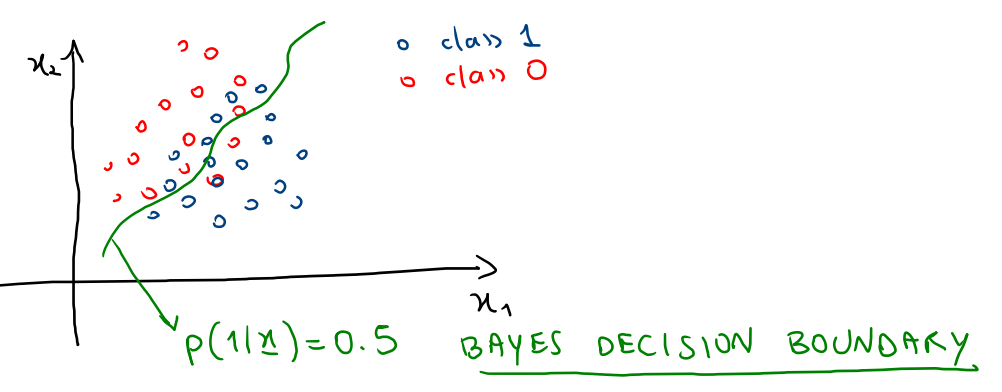
\includegraphics[width=0.6\textwidth]{BayesDecisionBoundary}
\end{figure}

    The \textbf{bayes error rate} (BER) is the probability of committing an error when classifying observations. It is defined as:
    
    $$\text{BER } = 1 - E_{\vec{X}}\left(\max_{j} p(j|\vec{x})\right)$$
    
(Since the class with the highest probability is the one considered for our observations, the probability of getting an error is equal to the toatl probability subtracted with the probability taken into account)

\begin{figure}[h]
\caption{The figure on the left represents the best possible scenario, as the BES value is 0, and the decision surface separate completely the elements belonging to the two classes. The graph on the left instead shows an intermadiate situation, where $ BER \neq 0 $}
\centering
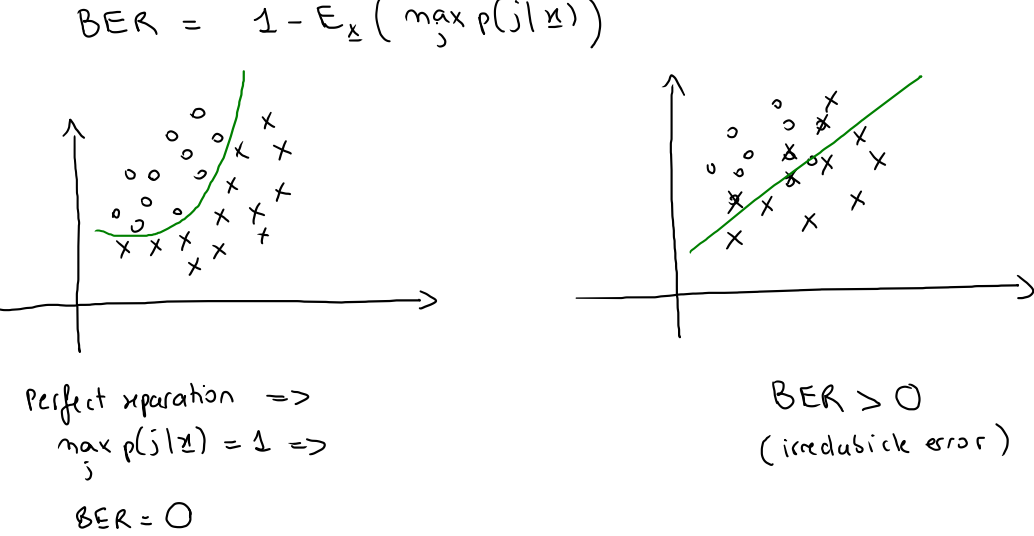
\includegraphics[width=0.6\textwidth]{BERBayesErrorRate}
\label{BER}
\end{figure}

    We talk about \textbf{perfect separation } of the classes when 
    $$\max_{j} p(j|\vec{x}) = 1 \implies \text{ BER } = 0$$
    In this case it is possible to classify any $\vec{x}$ without error (figure \ref{BER}). More often than not,
    $\text{BER } > 0$, therefore you have some irreducible error due to a partial overlap of the classes.

    It is possible to use a more generic loss function, called \textbf{misclassification loss function}, which can be represented (if $K = 2$) as:
    
\begin{table}
\centering
\caption{This is the table representing the possible values of $ L(Y, \hat{Y}(\vec{X})) $. $c_0$ and $c_1$ represent two different cost values}
\begin{tabular}{|l||c|c|}
	\hline
	\textbf{True, Predictions} & \textbf{0} & \textbf{1} \\
	\hline
	\hline
	\textbf{0} &  $0$ & $c_0$ \\
	\hline
	\textbf{\textbf{1}} & $c_1$ & $0$\\
	\hline
\end{tabular}
\end{table} 

    This loss function is analogous to the 0-1 loss function, but it assigns \textbf{different weights to different errors}, therefore the misclassifications have different costs:
    \begin{itemize}
      \item $C_0$ is the misclassification cost of misclassifying a class 0 to 1
      \item $C_1$ is the misclassification cost of misclassifying a class 1 to 0
    \end{itemize}
    Just like the 0-1 loss function, misclassification loss function can be generalized for $K$ classes.
    This loss function is generally better than the 0-1 loss function since\textbf{ in real situations it is likely for misclassifications to have different relevance} (credit risk evaluation, medical context and others). Moreover, this loss function allows you to adjust for unbalanced classes. Consider for example a rare disease; using a 0-1 loss function results in a model which always classifies patients as healty, therefore it is almost always correct, but it does not perform well when trying to determine which patients are affected by the disease. When using misclassification loss function, you can instead increase the weight of the misclassification "classify a patient as healthy when they are not", which may lead to worse results in terms of identifying healthy patients, but way better results in terms of identifying diseased patients.
    
    Repeating the same steps used for 0-1 loss function, we can determine the threshold for the misclassification function (for $k=2$ but it can be generalized)
    $$E[L(Y,0)] = c_1 p(1|\vec{x}) \text{ and } E[L(Y,1)] = c_0 p(0|\vec{x})$$
  
    Therefore we assign $\vec{x}$ to class 1 if 

    $$c_1 p(1|\vec{x}) > c_0 p(0|\vec{x})$$

    But since $p(0|\vec{x}) = 1 - p(1|\vec{x})$, we can instead write
    \begin{align*}
    c_1 p(1|\vec{x}) &> c_0 - c_0 p(1|\vec{x})) \\
    p(1|\vec{x}) &> \frac{c_0}{c_0 + c_1}
    \end{align*}
    which is the \textbf{classification threshold that takes into account different error weights}.

  \section{Model accuracy}
    In practice, we would use our chosen method to estimate $f(\vec{x})=E[Y|\vec{X}=\vec{x}]$ (regression) or $p(1|\vec{x})$ (classification) from training data $(\vec{x}_i, y_i), \; i = 1, \dots, n$.
    The \textbf{accuracy} of the model is typically measured on some \textbf{test data}
    $(\vec{x}_i^{(t)}, y_i^{(t)}), \, i = 1, \dots, m $.

    Therefore, a regression that uses MSE has for accuracy
    $$\text{MSE } = \frac{1}{m} \sum_{i = 1}^{m}\left(y_i^{(t)} - 
                    \hat{f}\left(\vec{x}_i^{(t)}\right)\right)^2$$
    
    
\begin{table}
\centering
\begin{tabular}{|l||c|c|}
	\hline
	\textbf{True,
		Predictions} & \textbf{0} & \textbf{1} \\
	\hline
	\hline
	\textbf{0} &  $ TN $ & $ FP $ \\
	\hline
	\textbf{\textbf{1}} & $ FN $ & $ TP $ \\
	\hline
\end{tabular}
\caption{Confusion matrix}
\label{ConfMat}
\end{table} 

    Meanwhile, for a classification, you create a \textbf{confusion matrix} (figure \ref{ConfMat}), estimate the probabilities via some method, substitute the values into the following formulas to obtain \textbf{sensitivity and specificity}.
     
    \begin{align*}
      \text{True positive rate (TPR)} &= \frac{\text{TP}}{\text{TP } + \text{ FN}} &
        &= \text{ \textbf{sensitivity}} \\\\
        
      \text{False positive rate (FPR)} &= \frac{\text{FP}}{\text{FN } + \text{ FP}} 
        &= 1 - \frac{\text{TN}}{\text{TN } + \text{ FP}} &= 1 - \text{ \textbf{specificity}} \\\\
        
      \text{Error rate} &= \frac{\text{FP } + \text{ FN}}{m}
    \end{align*}
    Notice that this last formula only works when using a 1-0 loss function; if you are using a misclassification loss function, the formula is similar but weighted:
    $$\text{Misclassification cost}= \frac{c_0 \text{ FP} + c_1 \text{ FN}}{m}$$

    Since defining the exact costs of the misclassifications might prove difficult, a possible approach is using the \textbf{Receiver Operating Characteristic (ROC) curve}. Basically you plot all the pairs (FPR, TPR) you obtain by varying the classification threshold from 0 to 1;
    you will then obtain a curve from which you can decide which value to use as a threshold (the one you see fit for your needs of specificity and sensibility). 
   
\begin{figure}[h]
\caption{Image taken from Wikipedia. ROC curve. }
\centering
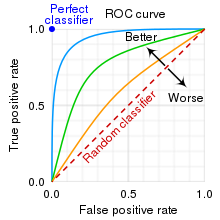
\includegraphics[width=0.6\textwidth]{RocCurve}
\label{ROCcurve}
\end{figure}

    Different models have different ROC curves.
    The best possible curve would touch the top left corner (figure \ref{ROCcurve}), meaning that you never misclassify any observation and therefore the model is deterministic.
    The worst possibile curve corresponds to the diagonal (from bottom left to top right corner), meaning that you have a 1/2 chance of misclassifying the observation (the same as tossing a coin to decide).
    The \textbf{area under the curve (AUC)} is the area between the curve and the main diagonal. Its value goes from $0$ in the worst case to $0.5$ in the best one. 
    For these reasons, you want a curve that is as high as possible (and thus has the biggest possible AUC). 
    When choosing between two models, if the ROC curve of one of the models is always above the ROC of the other model, the former one is the strictly better one; if the two ROC curves intersect, you choose the model whose curve in highest in the region you are most interested in (based on sensibility and specificity).    
  